\documentclass[11pt,a4paper]{article}
\usepackage[utf8]{inputenc}
\usepackage[T1]{fontenc}
\usepackage{amsfonts}
\usepackage[french]{babel}
\frenchbsetup{StandardLists=true} % à inclure si on utilise \usepackage[francais]{babel}
\usepackage{enumitem}
\usepackage{amssymb}
\usepackage{amsmath}
\usepackage[left=2cm,right=2cm,top=2cm,bottom=2cm]{geometry}
\usepackage{multirow}
\usepackage[dvipsnames]{xcolor}

\usepackage[T1]{fontenc}
\usepackage{fouriernc}
\usepackage{graphicx}

\usepackage{setspace}
\singlespacing

\usepackage{pstricks}
\usepackage{xkeyval}
\usepackage{pst-labo}


\usepackage{multicol}
\usepackage{caption}
\usepackage{fancyhdr}
\pagestyle{fancy}
\renewcommand\headrulewidth{1pt}
\fancyhead[L]{Lycée Denis Diderot }
\fancyhead[R]{Classe de Terminale}
\setcounter{page}{1}\fancyfoot[C]{page \thepage}
\fancyfoot[R]{Année 2025 2026}
\fancyfoot[L]{Alexis RUIZ}
\usepackage{multirow,tabularx,booktabs}
\newcommand{\cadreblanc}[1]{%
\medskip\framebox[\linewidth][c]{%
\rule{0mm}{#1mm}}\par
\medskip}

\usepackage{awesomebox}
\setlength{\aweboxvskip}{0mm}
\usepackage{pifont}
\usepackage{chemmacros}
\chemsetup{modules=all}

\renewcommand{\arraystretch}{2}
\newcommand*\acocher{\quitvmode{\fboxsep0pt \fboxrule0.8pt \fbox{\vrule height1.8ex depth.1ex width0pt \vrule height0pt depth0pt width1.9ex }}}

\newcommand{\defproblem}{\awesomebox[black]{2pt}{\rotatebox{90}{\large{\textbf{Problématique}}}}{black}}
\newcommand{\defconclusion}{\awesomebox[black]{2pt}{\rotatebox{90}{\Large{\textbf{Conclusion}}}}{black}}

\frenchbsetup{StandardLists=true}
\begin{document}



\center \LARGE{TP1 - Écrire une réaction d'oxydo-réduction}
\\[0,3cm]

\normalsize

\hrule\
\\[0,2cm]

\flushleft \textbf{NOM :\\
Prénom:\\[0,2cm]
}
\hrule\
\\[0,2cm]

\defproblem{\begin{minipage}{14cm}
{
Philippe va pulvériser de la bouillie bordelaise (composée de cuivre et de chaux éteinte) sur sa vigne pour la protéger de certaines maladies. Il la prépare dans un récipient en fer. N'ayant pas tout utiliser, il ferme le récipient. une semaine après, la bouillie bordelaise semble décolorée. \\
\begin{center}
\fbox{\textbf{Que s'est-il passé?}}
\end{center}
}
\end{minipage}}

\vspace {1cm}

\ding{202} Citer les deux éléments métalliques présents dans le récipient. \\
\cadreblanc{25}

\ding{203} Introduire dans un tube à essai propre un peu de fer en poudre à l'aide d'une spatule.\\[1cm]

\ding{204} Remplir le tube à essai à la moitié avec une solution de sulfate de cuivre (\ch{Cu\pch[2] + SO4\mch[2]})\\[1cm]

\ding{205} Boucher et secouer. Noter l'évolution sur les schémas ci dessous :\\[1cm]


\begin{center}
\psset{unit=0.8cm}
\psset{bouchon=true}
\pstTubeEssais[glassType=tube, niveauLiquide1=0]\hspace {3cm}
\pstTubeEssais[glassType=tube, niveauLiquide1=0]
\end{center}

\ding{206} Prélever un peu de liquide et l'introduire dans un autre tube à essai. \\[1cm]

\ding{207} Ajouter quelques gouttes d'hydroxyde de sodium \ch{NaOH} puis écrire la couleur du précipité observé. \\
\cadreblanc {15}

\newpage

\ding{208} A l'aide du tableau d'identification des ions présents ci-dessous, identifier l'ion présent dans la solution. 
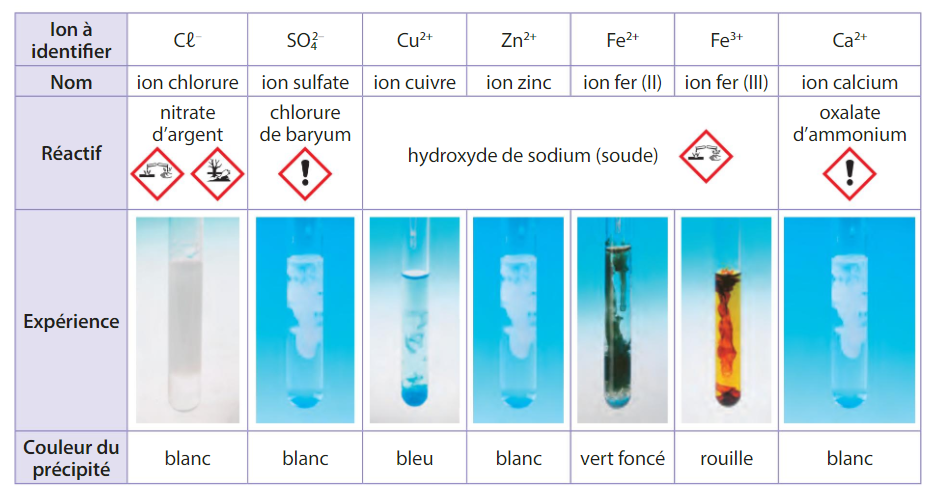
\includegraphics[scale=0.5]{images/tableau pp.png} 

\ding{209} Cocher l'ion métallique qui forme un précipité couleur marron-orange.
\begin{center}
$\Box$ fer \hspace{1cm} $\Box$ aluminium \hspace{1cm} $\Box$ cuivre \hspace{1cm} $\Box$ zinc 
\end{center}

\ding{210} L'élément cuivre initialement sous forme d'ions \ch{Cu\pch[2]}se transforme en cuivre métallique \ch{Cu}, ce qui se traduit par la demi équation équilibrée : 
\begin{reaction}
    Cu\pch[2] + 2 e- -> Cu
\end{reaction}
Écrire la demi-équation pour le fer : \dotfill 

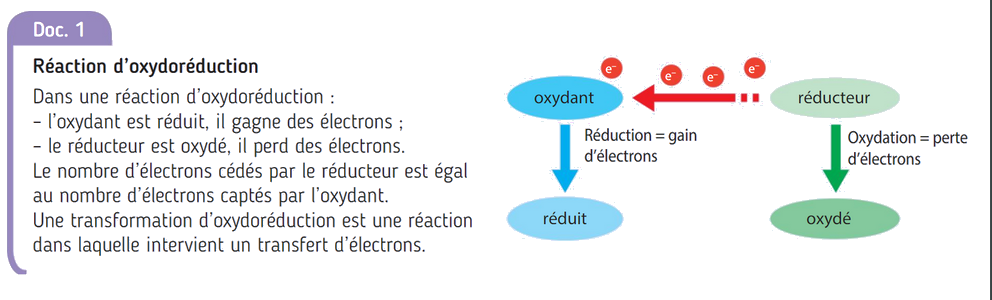
\includegraphics[scale=0.5]{images/Doc1.png} 
\ding{211} Lire le document et écrire la réaction d'oxydoréduction vue dans l'expérience :\\
\cadreblanc{10}
\dotfill
\vspace{0.5cm}
\defconclusion{\begin{minipage}{14cm}
{
Expliquer pourquoi il est déconseillé de stocker de la bouillie bordelaise dans du fer :\\
\cadreblanc{25}
}
\end{minipage}}



\end{document}